%# -*- coding:utf-8 -*-
\subsection[冠状动脉分割I]{基于CURVES的冠状动脉分割}

\begin{frame}
\begin{itemize}
\item \textbf{CURVES方法}
\end{itemize}
\end{frame}

\begin{frame}
\begin{itemize}
  \item \textbf{心脏区域的ROI提取}:
\end{itemize}
\begin{figure}[t]
\centering
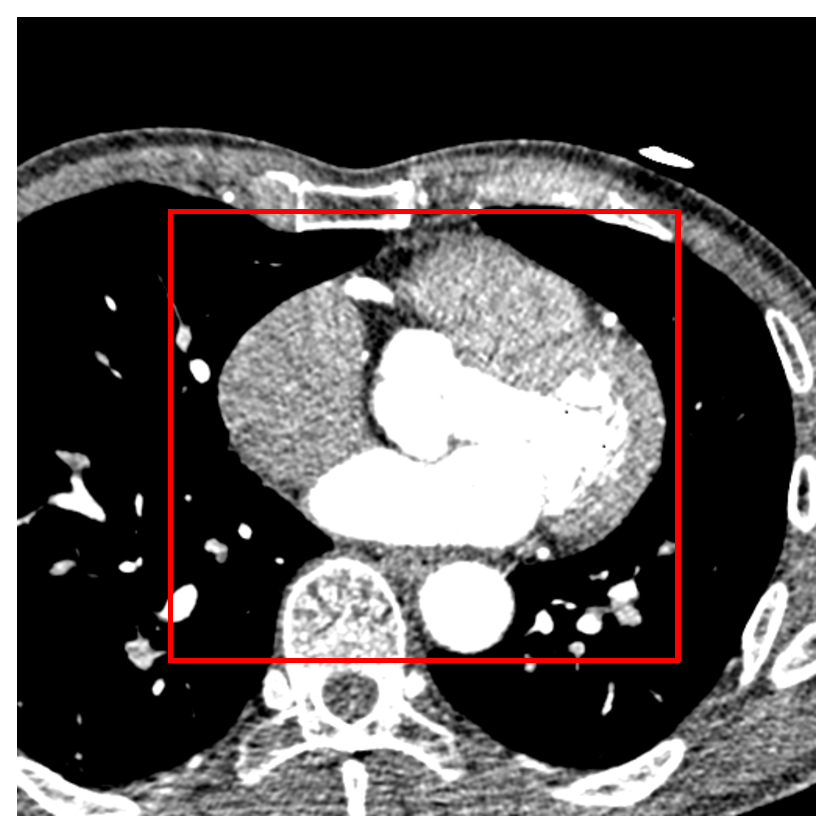
\includegraphics[width=1.5in]{../../Figures/coronary/ROI_Extraction}
% \caption[心脏区域的ROI提取]{心脏区域的ROI提取。}
% \label{fig:coronary_ROI}
\end{figure}
\end{frame}

\begin{frame}
\begin{itemize}
  \item \textbf{基于CURVES的冠状动脉分割流程}:
\end{itemize}
\begin{figure}[t]
\centering
%# -*- coding:utf-8 -*-
\begin{tikzpicture}[scale=.37]

\draw [black,thick,rounded corners] (-3,0) rectangle (3,2);            % binary threshold
\draw [black,thick,rounded corners] (-3,3) rectangle (3,5);  % CURVES

\draw [black,thick,rounded corners] (-8,7) rectangle (-2,9);   % initial contours

\draw [black,thick,rounded corners] (2,7) rectangle (8,9);     % feature images

\draw [black,thick,rounded corners] (-3,11) rectangle (3,13);  % thresholding
\draw [black,thick,rounded corners] (-3,14) rectangle (3,16);  % curvature anisotropic diffusion
\draw [black,thick,rounded corners] (-3,17) rectangle (3,19);  % raw input

\node [above right] at (-2.25,0.25) {\scriptsize \fs \bf 二值阈值滤波};
\node [above right] at (-2.25,3.25) {\scriptsize \fs \bf 测地活动轮廓};

\node [above right] at (-7.65,7.35) {\scriptsize \fs \bf 初始水平集演进};

\node [above right] at (2.82,7.35) {\scriptsize \fs \bf 特征图像计算};

\node [above right] at (-2.3,11.35) {\scriptsize \fs \bf 二值阈值滤波};
\node [above right] at (-2.9,14.35) {\scriptsize \fs \bf 曲率各向异性扩散};
\node [above right] at (-1.95,17.35) {\scriptsize \fs \bf ROI体数据};

\draw [<-,thick] (0,2) -- (0,3);

\draw [<-,thick] (0,5) -- (0,6);
\draw [thick] (-5,6) -- (5,6);
\draw [thick] (-5,6) -- (-5,7);
\draw [thick] (5,6) -- (5,7);

\draw [<-,thick] (-5,9) -- (-5,10);
\draw [<-,thick] (5,9) -- (5,10);
\draw [thick] (-5,10) -- (5,10);
\draw [thick] (0,10) -- (0,11);

\draw [<-,thick] (0,13) -- (0,14);
\draw [<-,thick] (0,16) -- (0,17);

\end{tikzpicture} 
% 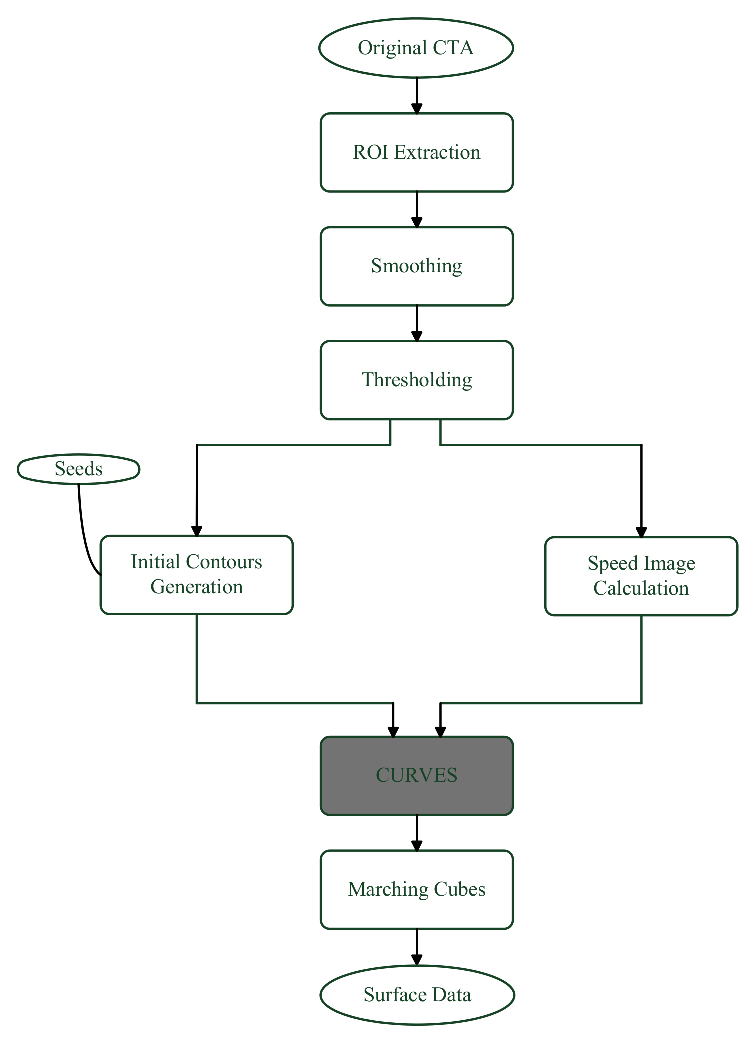
\includegraphics[width=3.2in]{Figures/coronary/DataFlow}
% \caption[心脏区域的ROI提取]{心脏区域的ROI提取。}
% \label{fig:coronary_ROI}
\end{figure}
\end{frame}

\begin{frame}
\begin{itemize}
  \item \textbf{预处理结果}:
  \begin{enumerate}
    \item 保护物体边缘的平滑处理($\text{传导参数} = 9.0$)
    \item 阈值滤波($\text{TH}_{\text{lower}} = 160$, $\text{TH}_{\text{upper}} = 600$
  \end{enumerate}
\end{itemize}
\begin{columns}[b,onlytextwidth]
\begin{column}{.5\textwidth}
\begin{figure}[t]
\centering
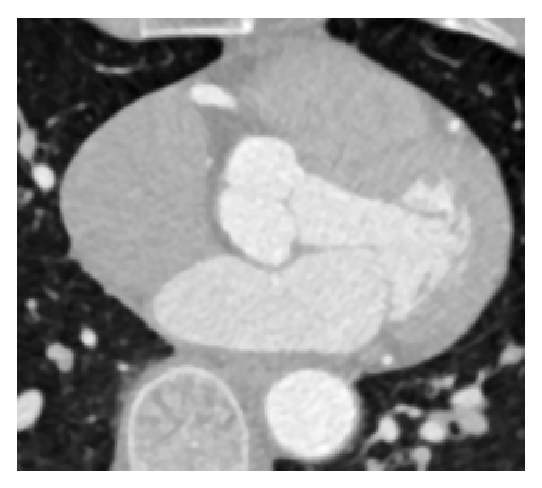
\includegraphics[height=1.5in]{../../Figures/coronary/smooth.eps}
\end{figure}
\end{column}
\begin{column}{.5\textwidth}
\begin{figure}[t]
\centering
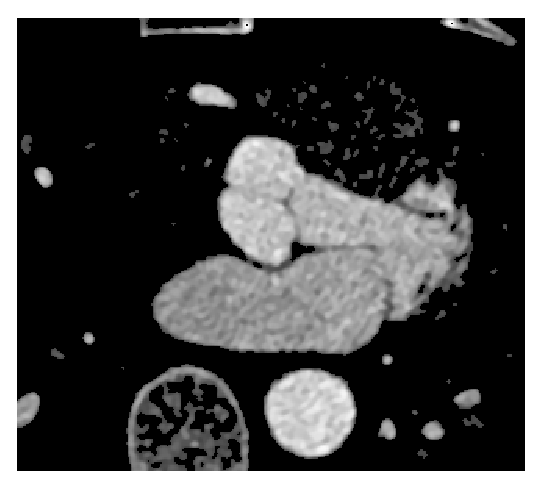
\includegraphics[height=1.5in]{../../Figures/coronary/threshold.eps}
\end{figure}
\end{column}
\end{columns}
\end{frame}

\begin{frame}
\begin{itemize}
  \item \textbf{特征图像计算}:
  \begin{enumerate}
    \item 基于Gaussian核运算所得到的梯度图像($\sigma = 0.9$)
    \item 通过S函数实现的像素亮度非线性映射($m = -80$, $n = 120$)
  \end{enumerate}
\end{itemize}
\begin{columns}[b,onlytextwidth]
\begin{column}{.5\textwidth}
\begin{figure}[t]
\centering
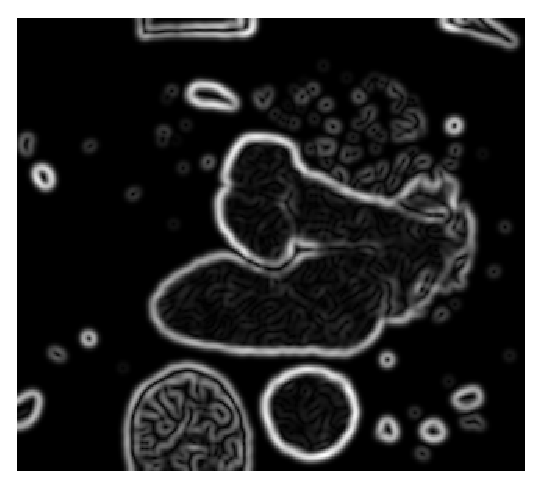
\includegraphics[height=1.5in]{../../Figures/coronary/gradient.eps}
\end{figure}
\end{column}
\begin{column}{.5\textwidth}
\begin{figure}[t]
\centering

\includegraphics[height=1.5in]{../../Figures/coronary/sigmoid.eps}
\end{figure}
\end{column}
\end{columns}
\end{frame} 

\begin{frame}
\begin{itemize}
  \item \textbf{水平集演进过程}:
  \begin{enumerate}
    \item 通过快速步进算法生成的初始水平集围线
    \item 由CURVES驱动的围线演进结果
    \item 对演进结果进行二值阈值滤波处理后的结果
  \end{enumerate}
\end{itemize}
\begin{columns}[b,onlytextwidth]
\begin{column}{.3\textwidth}
\begin{figure}[t]
\centering
\setlength{\fboxrule}{0.1pt}
\setlength{\fboxsep}{0cm}
\fbox{
\includegraphics[width=1.2in]{../../Figures/coronary/fastmarching.eps}}
\end{figure}
\end{column}
\begin{column}{.3\textwidth}
\begin{figure}[t]
\centering
\setlength{\fboxrule}{0.1pt}
\setlength{\fboxsep}{0cm}
\fbox{
\includegraphics[width=1.2in]{../../Figures/coronary/curves.eps}}
\end{figure}
\end{column}
\begin{column}{.3\textwidth}
\begin{figure}[t]
\centering
\setlength{\fboxrule}{0.1pt}
\setlength{\fboxsep}{0cm}
\fbox{
\includegraphics[width=1.2in]{../../Figures/coronary/final.eps}}
\end{figure}
\end{column}
\end{columns}
\end{frame} 

\begin{frame}
\begin{itemize}
  \item \textbf{冠状动脉表面模型}:
\end{itemize}
\begin{figure}[t]
\centering
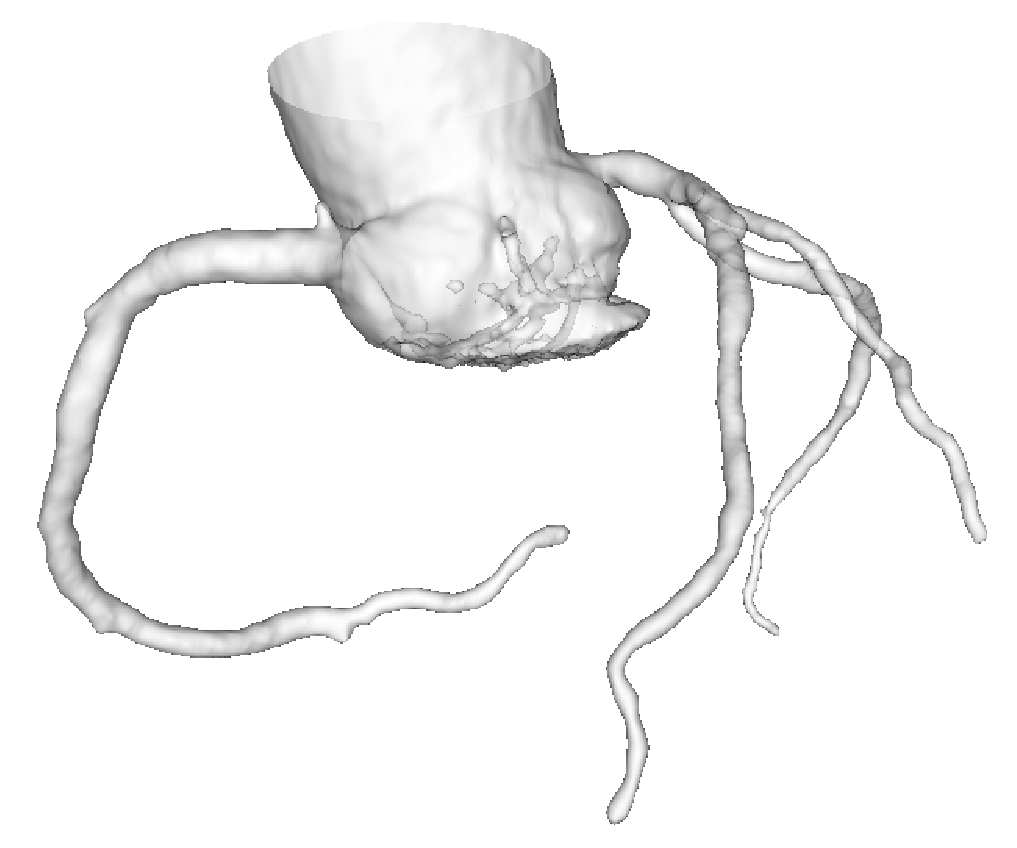
\includegraphics[width=1.5in]{../../Figures/coronary/model}
% \caption[心脏区域的ROI提取]{心脏区域的ROI提取。}
% \label{fig:coronary_ROI}
\end{figure}
\end{frame} 

\begin{frame}

\end{frame} 
